\chapter{Introdução}
\label{chp:introduction}

% \begin{quotation}[]{Poul Anderson}
% I have yet to see any problem, however complicated, which, when looked at in the
% right way, did not become still more complicated.
% \end{quotation}

Atividades relacionadas à vigilância, inspeção e controle, que hoje são 
realizadas por seres humanos, são candidatas a serem executadas por sistemas 
autônomos no futuro \citep{hernandez2013game}. Alguns exemplos dessas tarefas 
são: patrulhar fronteira de países ou muros de uma área civil, vigiar os 
corredores de um prédio, monitorar frotas marítimas e inspecionar áreas sujeitas 
a vazamentos de gás ou incêndios \citep{sampaiophd}.

Segundo a publicação \citep{hernandez2013game}, esses sistemas de segurança 
quando operados por humanos são, em sua maioria, previsíveis e inflexíveis, pois 
sua performance pode ser influenciada por fatores como o tédio, a distração ou a 
fadiga. Dessa forma, os autores afirmam que é importante melhorar os elementos 
de segurança desses sistemas para auxiliar seres humanos e destacam a Patrulha 
Multiagente \citep{Chevaleyre:2004:TAM:1018411.1019013} como um dos sistemas que 
pode fazer esse papel.

A Patrulha Multiagente pode ser definida como a tarefa de um agente que deve 
perceber uma porção limitada do ambiente e detectar eventos ou anomalias 
\citep{6315145}. Mais especificamente, pode ser definida como um problema no qual 
um time de indivíduos (agentes), visita tão frequentemente quanto possível, 
pontos de interesse contidos em uma área \citep{6495145}. Ou ainda como um 
problema de vigilância, onde deve-se minimizar o tempo entre visitas dos agentes 
aos locais importantes de um ambiente conhecido 
\citep{Pippin:2013:PBT:2480362.2480378}.

Existem algumas versões do problema que estendem essa definição, variando as 
características dos agentes e do ambiente. Dentre elas destacam-se: problema da 
patrulha em ambientes dinâmicos, isto é, o ambiente onde o agente se move muda 
ao longo da execução do agente \citep{6615158}. Outra variação leva em 
consideração que os agentes podem ter velocidades diferentes \citep{6900280}. 
Alguns autores trabalharam com o problema da patrulha onde os agentes não tem a 
mesma capacidade e operam em diferentes níveis de qualidade 
\citep{Pippin:2013:PBT:2480362.2480378}. Outros trabalham com agentes que 
possuem restrições de mobilidade \citep{6315145}. E há ainda uma variação onde a 
quantidade de agentes muda ao longo da execução, isto é, um determinado agente 
pode sair ou ser substituído por outro: são os chamados sistemas abertos 
\citep{6495145}.

Para estudar o problema, no entanto, esta pesquisa utilizará uma definição mais 
formal, precisa e abrangente do problema, que auxilie o pesquisador a enxergar 
a patrulha multiagente do ponto de vista matemático e a implementar soluções em 
aplicações de software. Assim, a definição técnica empregada no decorrer deste 
trabalho será a proposta por Sampaio \citep{sampaiophd}.

Segundo o autor, uma instância da Patrulha Multiagente Temporal, do inglês 
\ac{tmap}, é uma 7-tupla, $ \langle E, P, S, s_{0}, A, I, M \rangle $. O 
ambiente que o agente percebe é representado por um grafo 
\citep{Rosen:2002:DMA:579402}, $E$, onde os vértices representam os pontos de 
interesse, $P$, a serem visitados e as arestas representam os caminhos entre 
esses pontos. Na \figref{fig:graphexample}, visualiza-se um exemplo de ambiente 
para o problema da patrulha modelado como um grafo. O modelo demanda também o 
conjunto de estados possíveis da sociedade de agentes, $S$, e um estado inicial, 
$ s_{0} $, tal que $ s_{0} \in S $. É necessário ainda um conjunto de ações 
possíveis, $A$, que alteram o estado da sociedade de agentes. Essas ações podem 
tanto ser individuais (realizadas por um dado agente) quanto coletivas 
(realizada pela sociedade inteira). Cada ação é descrita segundo uma lista de 
pré-condições, um custo de tempo e as alterações que são aplicadas no estado 
após a ação concluir. É preciso também explicitar o intervalo de medição, ou o 
intervalo de tempo, $I$, em que os agentes terão seu desempenho mensurado. E, 
por fim, se faz necessário um conjunto de métricas, $M$, para avaliar os 
agentes.

\begin{figure}[tp]
	\caption[Exemplo de ambiente modelado em um grafo]{Exemplo de ambiente 
		modelado em um grafo}
	\centering
	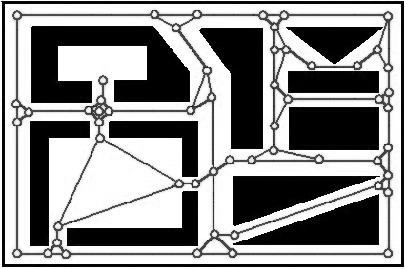
\includegraphics[width=0.75\columnwidth]{images/grafoExemplo.png}
	\caption*{Fonte: \citep{sampaiophd}}
	\label{fig:graphexample}
\end{figure}

Existem diversas métricas que podem compor o conjunto $M$. Um exemplo é o 
intervalo máximo que é definido como o maior intervalo entre visitas de todos os 
pontos de interesse \citep{sampaiophd}. Essa métrica é bastante utilizada em 
vários trabalhos da área \citep{6900280}, \cite{Pippin:2013:PBT:2480362.2480378}, 
\citep{Chevaleyre:2004:TAM:1018411.1019013}, \citep{6615158}. Outro exemplo, 
utilizado na literatura \citep{hernandez2013game}, é a ociosidade média, que 
consiste em calcular a média das ociosidades de cada ponto de interesse e depois 
tirar a média temporal desses valores.

Sendo assim, é possível concluir que o problema da Patrulha Multiagente é, 
fundamentalmente, um problema de otimização, onde é preciso escolher as ações 
dos agentes com a finalidade de minimizar (ou maximizar) uma dada métrica 
\citep{sampaiophd}.

Apesar de possuir diversas soluções com diferentes abordagens para o problema 
\citep{Chevaleyre:2004:TAM:1018411.1019013}, 
\citep{Machado:2002:MPE:1765317.1765332}, \citep{Almeida:2004:AAI}, 
\citep{4209122}, \citep{hernandez2013game}, soluções que utilizam estratégias 
evolucionárias \citep{Luke2013Metaheuristics} são pouco encontradas na 
literatura \citep{4630897}, \citep{6900280} e, por tanto, serão o objeto de 
pesquisa do presente trabalho.

\section{Objetivos Gerais}

Motivado pelos problemas descritos acima, este trabalho tem como objetivo geral 
a proposição e o estudo de soluções para \ac{tmap} utilizando estratégias 
evolucionárias. Outro objetivo é comprovar a eficácia e avaliar a relevância de 
abordagens evolucionárias para o problema da patrulha através de experimentos 
empíricos e da comparação destas soluções com as obtidas através de abordagens 
já propostas na literatura e tidas como tradicionais.

\section{Objetivos Específicos}

Tendo em vista tais objetivos gerais, este projeto visa atingir os seguintes 
objetivos específicos:

\begin{itemize}
	\item Investigar estratégias evolucionárias e como elas podem ser aplicadas 
		ao problema da patrulha multiagente temporal;
	\item Desenvolver um(s) algoritmo(s) baseado(s) em estratégias 
		evolucionárias para a solução da \ac{tmap};
	\item Implementar os algoritmos desenvolvidos em um simulador capaz de 
		computar diversas métricas para uma dada solução da \ac{tmap}.
	\item Avaliar o desempenho do algoritmo no simulador e verificar eficácia
		da abordagem.
	\item Comparar empiricamente as soluções encontradas com aquelas já 
		publicadas na literatura.
\end{itemize}